\documentclass[handout]{ximera}

\title{Post Video Questions}

\begin{document}

\begin{abstract}
\end{abstract}

% set 3 post

\maketitle

\begin{javascript}
  nameCheck = function(a,b) {
    return a.toLowerCase() != b.toLowerCase();
  };
\end{javascript}

Please answer each of these questions to the best of your ability. You are welcome to re-watch parts of any of the videos to help you.

The graph of the function f is shown below.

\begin{image}
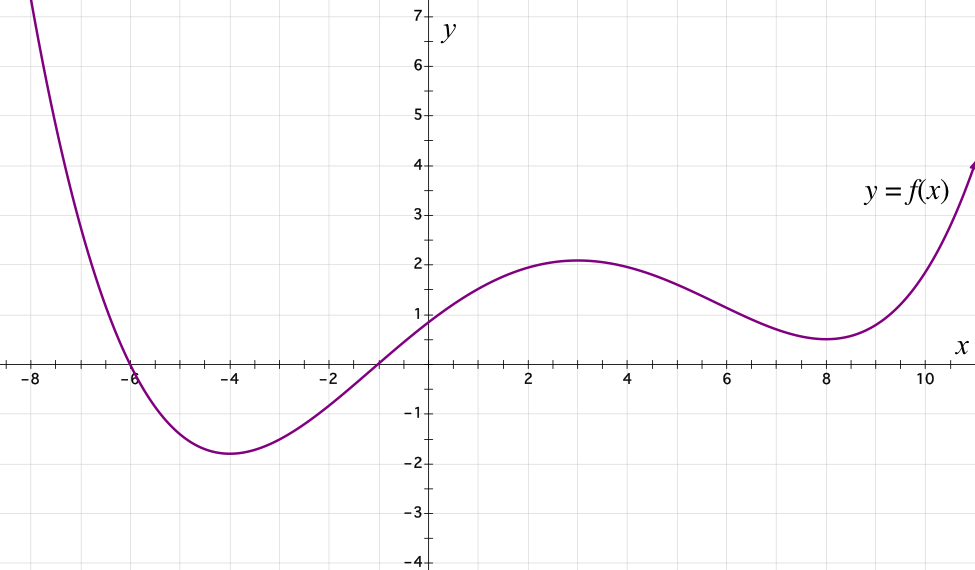
\includegraphics{Picture2.png}
\end{image}

\begin{problem}
For this problem, use the graph above.

\begin{enumerate}

\begin{tabular}{lr}

\begin{minipage}[t]{.5\textwidth}
\item On the interval $[-6, -4]$, is $f'(x)$:
\begin{multipleChoice}
\choice[correct]{$<0$}
\choice{$=0$}
\choice{$>0$}
\choice{more than one of the above}
\end{multipleChoice}
\end{minipage}

&

\begin{minipage}[t]{.5\textwidth}
\item On the interval $[-4, -2]$, is $f'(x)$:
\begin{multipleChoice}
\choice{$<0$}
\choice{$=0$}
\choice[correct]{$>0$}
\choice{more than one of the above}
\end{multipleChoice}
\end{minipage}

\\

\begin{minipage}[t]{.5\textwidth}
\item On the interval $[0, 2]$, is $f'(x)$:
\begin{multipleChoice}
\choice{$<0$}
\choice{$=0$}
\choice[correct]{$>0$}
\choice{more than one of the above}
\end{multipleChoice}
\end{minipage}

&

\begin{minipage}[t]{.5\textwidth}
\item On the interval $[2, 4]$, is $f'(x)$:
\begin{multipleChoice}
\choice{$<0$}
\choice{$=0$}
\choice{$>0$}
\choice[correct]{more than one of the above}
\end{multipleChoice}
\end{minipage}

\end{tabular}
\end{enumerate}
\end{problem}

\begin{problem}
For this problem, use the graph above.
\begin{enumerate}
\begin{tabular}{cc}

\begin{minipage}[t]{.5\textwidth}
\item On the interval $[-6, -4]$, is $f'(x)$:
\begin{multipleChoice}
\choice[correct]{increasing}
\choice{decreasing}
\choice{more than one of the above}
\end{multipleChoice}
\end{minipage}

&

\begin{minipage}[t]{.5\textwidth}
\item On the interval $[-4, -2]$, is $f'(x)$:
\begin{multipleChoice}
\choice[correct]{increasing}
\choice{decreasing}
\choice{more than one of the above}
\end{multipleChoice}
\end{minipage}

\\

\begin{minipage}[t]{.5\textwidth}
\item On the interval $[0, 2]$, is $f'(x)$:
\begin{multipleChoice}
\choice{increasing}
\choice[correct]{decreasing}
\choice{more than one of the above}
\end{multipleChoice}
\end{minipage}

&

\begin{minipage}[t]{.5\textwidth}
\item On the interval $[2, 4]$, is $f'(x)$:
\begin{multipleChoice}
\choice{increasing}
\choice[correct]{decreasing}
\choice{more than one of the above}
\end{multipleChoice}
\end{minipage}

\end{tabular}
\end{enumerate}
\end{problem}

\begin{problem}
For how many values of $x$ in the interval $[-8, 10]$ does $f'(x)=0$?
$\answer[format=integer]{3}$
\end{problem}

\begin{problem}
From following expressions, identify the smallest and largest according to the numerical value they represent:


\begin{tabular}{cc}

\begin{minipage}[t]{0.5\textwidth}
Largest:
\begin{multipleChoice}
\choice{$f'(8)$}
\choice[correct]{$\dfrac{f(8+\Delta x)-f(8)}{\Delta x}$ for $\Delta x > 0$}
\choice{$f(-6)$}
\choice{$f'(-6)$}
\end{multipleChoice}
\end{minipage}

&

\begin{minipage}[t]{0.5\textwidth}
Smallest:
\begin{multipleChoice}
\choice{$f'(8)$}
\choice{$\dfrac{f(8+\Delta x)-f(8)}{\Delta x}$ for $\Delta x > 0$}
\choice{$f(-6)$}
\choice[correct]{$f'(-6)$}
\end{multipleChoice}
\end{minipage}

\end{tabular}
\end{problem}

\end{document}